% This file was created with tikzplotlib v0.10.1.
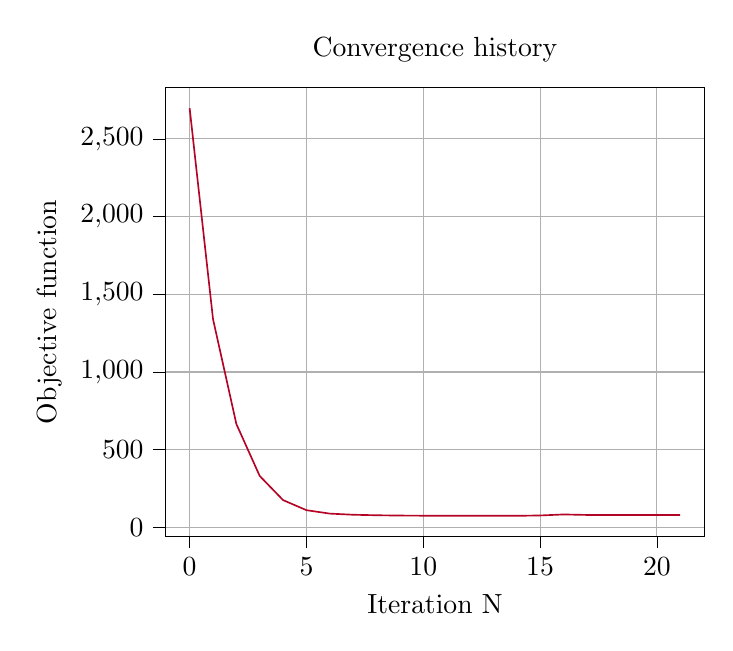
\begin{tikzpicture}

\definecolor{darkgray176}{RGB}{176,176,176}
\definecolor{firebrick180438}{RGB}{180,4,38}

\begin{axis}[
tick align=outside,
tick pos=left,
title={Convergence history},
x grid style={darkgray176},
xlabel={Iteration N},
xmajorgrids,
xmin=-1.05, xmax=22.05,
xtick style={color=black},
y grid style={darkgray176},
ylabel={Objective function},
ymajorgrids,
ymin=-56.1878564045003, ymax=2827.69991519705,
ytick style={color=black}
]
\addplot [semithick, firebrick180438]
table {%
0 2696.61410739698
1 1340.69719975026
2 665.295719944366
3 330.953397012819
4 175.94409133933
5 111.105831059072
6 89.0350154260762
7 81.7528610174375
8 78.4724355397695
9 76.5690624015191
10 75.6930548900034
11 75.2688746191894
12 75.0569196808242
13 74.9509416632314
14 74.8979513955702
15 77.1286339099154
16 83.6422082877931
17 80.4959121983754
18 79.8995252722031
19 79.8771090401021
20 79.8770766684397
21 79.877076668372
};
\end{axis}

\end{tikzpicture}
